\documentclass[11pt]{article}
\usepackage[margin=1in]{geometry}
\usepackage[T1]{fontenc}
\usepackage{lmodern}
\usepackage{amsmath,amssymb}
\usepackage{booktabs}
\usepackage[numbers,sort&compress]{natbib}
\usepackage[hidelinks]{hyperref}
\usepackage{graphicx}
\usepackage[font=footnotesize,skip=3pt]{caption}
\sloppy

\title{When the completeness of an agent's log is estimable:\\five pre-registered studies of capture-recapture over agent logs}
\author{Caio Theodoro}
\date{November 2026}

\begin{document}
\maketitle

\begin{abstract}
An audit of an AI agent assumes that its log is whole. Receipts and hash chains show that
a log was not altered, not that it is complete. Where one trusted counter numbers every
action at the source or the sink, the count should be read from it. This paper asks when
completeness is estimable where no such counter can exist, by capture-recapture over
several incomplete logs. Four pre-registered studies on recorded agent episodes with
simulated loss map where the estimate fails. It needs exact record linkage. It breaks
when loss depends on the action or comes in bursts (coverage 0.187 and 0.559 against a
bar of 0.90). It needs every channel an action can take to be itemised by two logs or
more (0.759 when an agent ran 0.856 of its actions through a batch tool that no log
itemised). A fifth study registered one estimator with a named model and replayed
sessions recorded from two models through a live rig: two uncoordinated originators, two
planes, and telemetry relays that are killed and restarted, in 420 registered runs. The
registered criterion passed on the runs left: the interval held the true count in 269 of
277 runs of the primary condition (Wilson 0.944 to 0.985), against the author's
registered prediction that it would not. 23 of the 300 planned runs were set aside on
integrity, and with those counted as not covered it is 269 of 300, whose Wilson interval
(0.857 to 0.926) straddles the bar, a reading of ``not shown''. The bound treats runs as
independent although they replay shared sessions, an interval with no upper end would
have counted as covering (none occurred), and this is one rig. The estimate was closer to
the true count than a sequence-gap baseline in 223 of the 277 runs. Without the end-state
witness the estimate covered 10 of them.
\end{abstract}

\section{The question}
\label{sec:question}

Audit regimes that reach AI agents start from a log~\citep{euaiact}. The engineering
around the log asks whether a line was changed after it was written: hash chains,
notarised channels, tamper-evident logs replayed by
witnesses~\citep{flightrecorder2026,vet2025,haeberlen2007peerreview}. These show that a
log was not altered. They do not show that it is complete: a line never written leaves
no trace in a chain.
Agents have deleted their own trace events when asked, and unprompted when it raised
their reward~\citep{qin2026tamper}, and ordinary telemetry loses records with no
adversary at all (\S\ref{sec:s5results}).

\paragraph{If a counter exists, read it.} Where one trusted counter numbers every action
at the source or at the sink and its last number can be read, the count is that number
and no estimate is needed. Where the numbers survive only on the records that survive,
the gaps give the losses inside the sequence and the lost tail has to be estimated. On
recorded episodes with simulated loss (Table~\ref{tab:earlier}, lower block), that
tail-corrected counter covered 0.944 at a mean width of 26.2 actions under loss that
falls on records one by one, against 0.952 at 38.9 for the three-log estimate. When loss
fell harder on the operations one log cannot see, it covered 0.952 and the estimate
0.254. It covered 0.000 when records were lost in blocks, and 0.002 when 5\% of actions
bypassed the gateway and took no number. So the counter is the better instrument where
it sees every action and records are lost independently of one another, and it fails
where loss comes in blocks or an action can go round it.

\paragraph{Where no counter can exist.} This paper is about the other setting: actions
come from several processes that share no numbering, the logs belong to components that
lose records on their own, and no single log is trusted to be whole. There the actions
missing from every log are a hidden population, and overlapping several incomplete
registers estimates what all of them missed~\citep{fienberg1972,bird2018mse}. I found no
work that applies this to an agent's log. The closest, capture-recapture over LLM judges
counting label errors, produced valid intervals too wide to beat a raw
count~\citep{kansal2026labels}. Elsewhere the method's known failure point is dependence
between the
lists~\citep{eick1992inspection,petersson2004inspection,bohme2018stads,moore2007phish},
and the count is not identified without an assumption the data cannot
test~\citep{aleshinguendel2024}. So the question is under which conditions the estimate
can be relied on, and what it looks like when they fail.

\paragraph{The answer in brief.} Five pre-registered studies give six conditions
(\S\ref{sec:when}): no counter can be read; records are linked exactly; every channel is
itemised by two logs or more; one witness is of another kind than the rest; what the
logs lose together is as visible to that witness as the rest; and the interval allows
for loss in blocks. Four studies found the failures. In the fifth, with a real pipeline
losing the records, the registered interval held the true count in 269 of the 277 runs
left of the primary condition, which meets the registered criterion. 23 of
the 300 planned runs were set aside on integrity, and with those counted as not covered
it is 269 of 300, whose Wilson interval straddles the 0.90 bar and reads ``not shown''
(\S\ref{sec:s5results}). None of the six conditions can be checked from the estimate.
They are checked by reviewing the design.

\section{Terms and method}
\label{sec:method}

An \emph{action} is a tool call that changes the environment's state or sends data out.
The environment kernel appends one ledger entry per action, so the true count $N$ is a
program's output that no witness and no estimator reads. A \emph{witness} is a log that
records some of the actions. A \emph{channel} is a route an action can take: a direct
tool call, or a batch tool that runs a script of many operations in one call. A log
\emph{itemises} a channel if it holds one record per action taken through it.

\paragraph{Estimates.} Capture-recapture cross-classifies the actions by which witnesses
recorded them and estimates the cell nobody recorded. Studies 1 to 4 use
\texttt{ll\_bic}: Poisson log-linear models of the three-log table~\citep{fienberg1972},
pairwise interactions chosen by BIC, a 95\% profile-likelihood interval, no three-way
interaction. Study 5 registers \texttt{ll\_sa\_hom} (\S\ref{sec:s5design}).

\paragraph{Scoring.} \emph{Coverage} is the share of replicates (studies 1 to 4) or of
runs (study 5) whose 95\% interval holds $N$. Every registration sets the bar at 0.90
and was frozen in a commit before the runs it governs were made (the decision log gives
the times and the clocks). \emph{Post hoc} marks every result outside a registration.

\paragraph{Floors.} Every table of estimates carries three counts that need no model:
\texttt{trust\_trace}, the agent's own log taken as complete; \texttt{union\_count}, the
distinct actions in any log, with no interval; and \texttt{union\_bound}, the same
number as a lower bound with no upper end, which always covers and never bounds.

\section{Studies 1 to 4: where the estimate fails}
\label{sec:earlier}

The first four studies ran a live agent (\texttt{deepseek-v4.1-flash}; study 4 adds
\texttt{qwen3.8-flash}) on a back-office queue, an infra queue and a batch-tool variant
of the first. Three witnesses saw the actions: the harness's trace, a gateway proxy log,
and an end-of-shift diff of the environment's state with its outbound mail sink. Loss
was simulated afterwards on the complete logs: each replicate resamples the recorded
episodes, drops log lines by a loss model and estimates $N$ again.
Table~\ref{tab:earlier} gives each study's registered cell.

\begin{table}[!tb]
\centering\small
\resizebox{\linewidth}{!}{\begin{tabular}{llrrrrr}
\toprule
cell & linkage & \texttt{ll\_bic} & sequence counter & \texttt{trust\_trace} & \texttt{union\_count} & \texttt{union\_bound} \\
\midrule
study 1, back-office & signature & 0.940 (42.0) & -- & 0.000 & 0.000 & 1.000$^{\infty}$ \\
study 2, infra & signature & 0.300 (55.8) & -- & 0.000 & 0.000 & 1.000$^{\infty}$ \\
study 3, batch tool no log itemises & call id & 0.759 (333.6) & 0.000 (32.8) & -- & 0.000 & -- \\
study 3, reference pool, no batch tool & call id & 0.946 (39.0) & 0.954 (26.1) & -- & 0.000 & -- \\
study 4, second model, batch tool & call id & 0.200 (4780.8) & 0.069 (330.5) & -- & 0.000 & -- \\
\midrule
per-record loss & ledger id & 0.952 (38.9) & 0.944 (26.2) & 0.000 & 0.000 & 1.000$^{\infty}$ \\
loss on unseen operations, 1.2 times & ledger id & 0.254 (45.5) & 0.952 (28.6) & 0.000 & 0.000 & 1.000$^{\infty}$ \\
loss in blocks of 12 actions & ledger id & 0.574 (49.1) & 0.000 (19.3) & 0.000 & 0.000 & 1.000$^{\infty}$ \\
session quality shared by all three logs & ledger id & 0.194 (101.8) & 0.480 (25.7) & 0.000 & 0.000 & 1.000$^{\infty}$ \\
5\% of actions bypass the gateway & ledger id & 0.926 (40.8) & 0.002 (26.2) & 0.000 & 0.000 & 1.000$^{\infty}$ \\
\bottomrule
\end{tabular}}
\par\smallskip{\footnotesize Coverage of the 95\% interval (mean width in actions for the two estimates); the bar in every registration is 0.90. Upper block: the registered cell of each of the first four studies, logs thinned at \texttt{fin\_mid} (infra: \texttt{transfer\_mid}); 100 replicates at the registered seed in studies 1 and 2, 3000 over 30 loss seeds in studies 3 and 4. Lower block: post hoc, the study-1 episodes, 500 replicates a row. The sequence counter is the tail-corrected one: an action's number is its position in the gateway's complete log, the counter is never lost, only the records it numbered, and an action that bypasses the gateway takes no number. --: not computed in that artifact. $^{\infty}$: every interval has no upper end. Sources: \texttt{artifacts/thinning/\{confirm,transfer\}.json}, \texttt{artifacts/robustness/bypass-analysis-\{bypass-llm,confirm\}.json}, \texttt{study4-adversary-s4-qwen-bypass.json}, \texttt{baselines.json}.}

\caption{Studies 1 to 4 and the post hoc loss cells: coverage of \texttt{ll\_bic}, of a
tail-corrected sequence counter where it was computed, and of the three floors.}
\label{tab:earlier}
\end{table}

\paragraph{Linkage (studies 1 and 2).} Study 1 passed at its registered seed (0.940)
and did not hold up: over 30 fresh loss seeds coverage is $0.893 \pm 0.006$. Study 2
predicted that the infra environment would fail, and it did (0.300, and 0.401 over 20
seeds). The cause was the registered linkage. Matching records by their effect pairs
records of different actions, and the false overlap reads as dependence between the
logs. Matched by the ledger id, which no auditor has, coverage is 0.948 and 0.946.
Post hoc, a call id that the harness writes into both the trace and the gateway restores
the back-office figure (0.946) and not the infra one (0.859), because the end-state diff
carries no id. The id is only as good as the lines: 5\% of lines duplicated in all three
logs take coverage to 0.094, and 5\% forged in all three to 0.000.

\paragraph{Loss that depends on the action, or comes in blocks (post hoc).} With exact
matching, a tenth more loss on the operations the end-state diff cannot see takes
coverage to 0.647 and a fifth more to 0.187, on intervals barely wider than before.
Loss in blocks of 12 consecutive actions takes coverage to 0.559 in back-office and
0.802 in infra. An interval widened by the dispersion between
episodes~\citep{wedderburn1974quasi,mccullagh1989glm} restores 0.952 and 0.994 there, at
2.5 to 3 times the width.

\paragraph{A channel no log itemises (study 3).} The third study added a batch tool. The
ledger gets each inner action; the trace and the gateway log one call holding the script
text, and by stipulation no witness parses it. The agent ran 0.856 of its 1283 actions
through the tool, against a predicted 0.05 to 0.30. Coverage fell to 0.759 against
0.946 on a reference pool with no batch tool, on intervals 333.6 wide
against 39.0. The estimator still reported a gap in 0.995 of replicates, as it does in
every replicate of the reference pool, so a detected gap does not say that a channel is
unseen. Post hoc, one record per scripted action, taken from the ledger, restores 0.949.

\paragraph{Itemising is not enough (study 4).} The fourth study parsed the scripts from
their logged text. When a log drops a script's lines together, coverage is 0.469 where
the same records lost one by one give 0.952, 0.610 against 0.940 under an adversary
prompt, and 0.335 against 0.941 on a second model. That model routed 0.970 of its
actions through the batch tool and coverage fell to 0.200. The adversary prompt told the
agent how it is counted and asked it to undercount. It split the pool (11 of 23 episodes
used no script, against 1 under the neutral prompt), and no episode found a route beyond
the one channel. That adversary was weak: one episode, black box, the channel not named.
8 of study 4's 12 predictions held in full.

\paragraph{What these four leave open.} All loss was simulated, and in the first two
studies one gateway saw every action, so a counter could have existed. Study 5 removes both.

\section{Study 5: design}
\label{sec:s5design}

Study 5 (signed tag \texttt{prereg-study5}) asks three questions. Q1: does the interval
cover the true count when records are lost by real telemetry components, in blocks, to
both planes at once (criterion P1)? Q2: is the estimate closer to the true count than
counting sequence gaps, and than counting the union of the logs (P2, against each)? Q3
asks the same without the end state, and was predicted to fail.

\paragraph{The rig.} Two originators replay recorded sessions over MCP and share no
counter. Plane A goes through an unmodified open-source gateway, \texttt{agentgateway},
and plane B straight to an MCP front. One kernel service keeps the ledger. Each plane
has three witnesses. \texttt{spans} are the originator's own OpenTelemetry spans, sent
through a relaying collector; a batch is given up when the relay is away past the SDK's
retries. \texttt{access} is the receiver's access log, tailed by a second relaying
collector; lines written while that relay is away are skipped. \texttt{env} is the end
state and the outbound sink, each row with its last writer; an action overwritten or
undone later leaves nothing in it. Every SDK and collector setting is its default, no
code in the repository drops a record, and only the two relays and the originators are
ever killed. Both planes' spans pass one relay and both planes' access logs the other.
\texttt{spans} and \texttt{access} are linked by trace id and JSON-RPC id, both stamped
by the client library where no model output reaches them; \texttt{env} attaches by what
the action was. The single kernel is
itself a census at the sink. It stands for several downstream systems whose logs are not
collected, which the study stipulates and does not show.

\paragraph{Sessions and runs.} Sessions were recorded once from two models
(Table~\ref{tab:pools}), ticket by ticket, on a task mix in which later tickets correct,
revert, delete or rewrite what earlier ones did, which is what makes the end state blind
to part of the work. The pools were recorded before the freeze because their hashes are
part of what is frozen, and no run replayed them before the tag. A run replays 24 sessions drawn without replacement from one pool, with session starts spread
over 100 s, each call made when the recording made it. The plan is 420 runs in three
conditions (Table~\ref{tab:conditions}). \texttt{s1}, the primary condition, kills both
relays together at a time drawn from 8 to 90 s and restarts them 15 to 45 s later. It
includes the outage lengths at which a pilot had seen the estimator miss. A run is made
once and a run set aside is not replaced. The analysis ran once, after every run had a
folder and a hash of each folder was committed.

\begin{table}[!tb]
\centering\small
\resizebox{\linewidth}{!}{\begin{tabular}{lllrrrrrrrr}
\toprule
pool & plane A & plane B & sessions & actions & hidden & runs left & \texttt{ll\_sa\_hom} & \texttt{trust\_trace} & \texttt{union\_count} & \texttt{union\_bound} \\
\midrule
\texttt{ds} & \texttt{deepseek-v4-1-flash-1017} & \texttt{deepseek-v4-1-flash-1017} & 72 & 994 & 0.384 & 92 & 89 & 0 & 0 & 92 \\
\texttt{glm} & \texttt{zai-glm-5-3} & \texttt{zai-glm-5-3} & 72 & 1001 & 0.409 & 94 & 91 & 0 & 0 & 94 \\
\texttt{mix} & \texttt{deepseek-v4-1-flash-1017} & \texttt{zai-glm-5-3} & 72 & 999 & 0.395 & 91 & 89 & 0 & 2 & 91 \\
\bottomrule
\end{tabular}}
\par\smallskip{\footnotesize Actions: ledger actions as recorded. Hidden: one minus the rows the end state holds over the actions. Runs left: of the 100 \texttt{s1} runs planned on each pool. Last four columns: runs left whose interval holds the true count, reported as registered with no criterion; a pool is one model pairing on its own ticket seeds, and no conclusion is drawn by pool. Sources: \texttt{pool.json}, \texttt{registered.json} and \texttt{confirm.json} under \texttt{artifacts/study5}.}

\caption{Study 5: the pools of recorded sessions, and coverage by pool with the floors.}
\label{tab:pools}
\end{table}

\begin{table}[!tb]
\centering\small
\resizebox{\linewidth}{!}{\begin{tabular}{lp{5.6cm}rrrrrrr}
\toprule
 & stress & planned & set aside & left & in no log & spans & access & union exact \\
\midrule
\texttt{s0} & no stress & 60 & 2 & 58 & 0.000 & 0.000 & 0.000 & 58 \\
\texttt{s1} & both relays killed together, restarted together 15 to 45 s later & 300 & 23 & 277 & 0.068 & 0.190 & 0.300 & 2 \\
\texttt{s2} & each relay on its own outage; one originator killed for good & 60 & 9 & 51 & 0.029 & 0.311 & 0.273 & 18 \\
\bottomrule
\end{tabular}}
\par\smallskip{\footnotesize Study 5, the 420 registered runs. Set aside: failed the integrity check, applied before any test; a run is made once and not replaced. In no log: mean over the runs left of the share of a run's actions that no witness recorded. Spans, access: mean share of a plane's actions the telemetry witness missed. Union exact: runs left in which the logs together hold every action. Sources: \texttt{artifacts/robustness/study5-verdicts.json}, \texttt{artifacts/study5/confirm.json}.}

\caption{Study 5: the three registered conditions, the runs set aside by reason, and
what each condition lost.}
\label{tab:conditions}
\end{table}

\paragraph{The registered estimator.} \texttt{ll\_sa\_hom} sums the two planes' tables
and names one model in advance. Its point is Lincoln--Petersen between two lists, any
telemetry (spans or access) and the end state: the count seen, plus the actions seen by
the end state alone times those seen by telemetry alone, over those seen by both. That is
the maximum-likelihood missing cell of the log-linear model whose only interaction is
between spans and access. The interval is that model's profile likelihood with its cutoff
scaled by the dispersion between the run's session-and-plane tables, at a nominal level
of 95\%. Nothing is selected. The estimator and the restart condition were both chosen
after the first round of a pilot had been seen; the registration lists what was seen.

\paragraph{Baselines and criteria.} \texttt{seq\_gap\_tail} reads the JSON-RPC ids on
the delivered telemetry of each session and plane, counts the ids missing up to the last
one seen, converts requests to actions at the share of seen calls that were actions, and
adds the expected lost tail. It is told each session's first id and is not shown the end
state. P1 passes if the Wilson 95\% lower end of coverage over the \texttt{s1} runs left
is at or above 0.90 and under 0.05 of intervals are unbounded; an interval with no upper
end counts as covering unless its lower end is above the truth. P2 passes against a
baseline if the exact one-sided 97.5\% lower bound on the share of runs in which the
point is strictly closer to the true count is above 0.5, a tie counting as a loss. A
fail reads ``missed'' when the interval excludes meeting the criterion and ``not shown''
otherwise. Two gates come first: fewer than 270 \texttt{s1} runs left is
``underpowered'', and a mean share of actions in no log under 0.02, or telemetry that
loses under 0.01 of a plane's actions, is ``not exercised''.
An integrity check sets a run aside before any test (Table~\ref{tab:conditions}).

\paragraph{Predictions.} The registration predicted that P1 would not be met on its
coverage clause. The basis was the pilot: 18 of 20 runs covered on recorded sessions
(Wilson 0.699 to 0.972) and 23 of 24 on scripted ones (0.798 to 0.993), which with a
flat prior gave a pass a probability of 0.165 and 0.494. With all 300 runs left the bar
asks for 281 covered. Table~\ref{tab:predictions} lists the other predictions.

\section{Study 5: results}
\label{sec:s5results}

All 420 runs were made, their folders hashed, and the analysis run once. Every verdict
below is read from the verdict artifact that run wrote.

\paragraph{Runs set aside, and the gates.} The integrity check set aside 34 runs: 2 of
60 in \texttt{s0}, 23 of 300 in \texttt{s1} and 9 of 60 in \texttt{s2}
(Table~\ref{tab:conditions}), most of them for a call made late. None of the 23 in
\texttt{s1} is of the two kinds the registration says can follow from the loss under
study (an empty witness file, an access log with no line delivered). The runs set aside
were bunched in the plan's order and not spread over it. Docker Desktop quit once during
the study; the run under way, \texttt{s5-s1-230}, was lost to it and is among the 23.
The cause of the lateness is not established, and whether the runs set aside would have
been covered is not known. The share set aside is lower with no stress than under it, so
that none of the 23 is of those two kinds does not make being set aside independent of
the loss. The registered answer is the figure below with all 23 counted as not covered,
and no other is offered. Neither gate fires: 277 \texttt{s1} runs are left against a
bar of 270, and the mean share of a run's actions in no log is 0.068. An \texttt{s1}
run has 316 to 353 actions (Table~\ref{tab:conditions}).

\paragraph{P1.} The criterion as registered is met on the runs left:
\texttt{ll\_sa\_hom} covered 269 of 277 \texttt{s1} runs (Wilson 0.944 to 0.985) and no
interval was unbounded, so both clauses read ``pass''. 23 of the 300 planned \texttt{s1}
runs were set aside on integrity, and with those counted as not covered it is 269 of
300, Wilson 0.857 to 0.926, which straddles the 0.90 bar and reads ``not shown''. The
registration gives that second figure no criterion and puts it beside the verdict. The
pass is therefore not one that survives counting the runs set aside against it. Three
caveats are fixed by the registration. The bound treats runs as independent, and the 100
planned runs of a pool draw 24 of the same 72 sessions, so the bound is too narrow by an
amount the study does not measure. This is one rig. And an interval with no upper end
would have counted as covering; none occurred in \texttt{s1}, so coverage over bounded
intervals alone is the same count. Of the eight runs not covered, seven intervals end
below the true count, by 1 to 5 actions, and one starts 9 above it
(Figure~\ref{fig:s5}a). The pilot's misses are reported beside the verdict, as
registered. On recorded sessions: \texttt{ptr-ds-restart-6} (325 actions, interval 326
to 342) and \texttt{ptr-ds-restart-7} (330, interval 326 to 327). On scripted sessions:
\texttt{pt3-node-restart-0} (372, interval 367 to 369).

\begin{figure}[!tb]
\centering
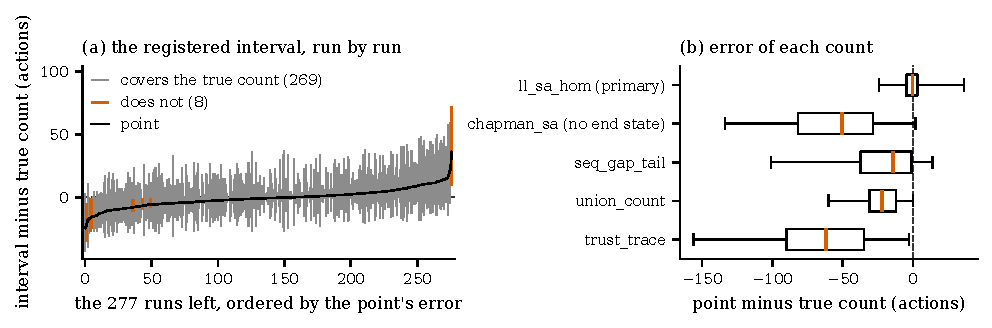
\includegraphics[width=\linewidth]{figures/fig_study5.pdf}
\caption{Study 5, the 277 \texttt{s1} runs left. (a) Each \texttt{ll\_sa\_hom} interval
minus the true count. (b) Each count's error; boxes are quartiles, whiskers the range.
Both display the per-run records and are not part of the registered analysis.}
\label{fig:s5}
\end{figure}

\begin{table}[!tb]
\centering\small
\resizebox{\linewidth}{!}{\begin{tabular}{llrrrrrrrr}
\toprule
method & role & covered & Wilson 95\% & unbounded & width & abs.\ error & error & closer than \texttt{seq\_gap\_tail} & closer than \texttt{union\_count} \\
\midrule
\texttt{ll\_sa\_hom} & primary & 269 & 0.944 to 0.985 & 0 & 32.0 & 3.9 & $-$0.5 & 223 & 261 (3) \\
\texttt{ll\_sa\_hom\_sig} & primary, no id trusted & 269 & 0.944 to 0.985 & 0 & 32.0 & 3.9 & $-$0.5 & 223 & 261 (3) \\
\texttt{ll\_bic\_hom} & beside it & 262 & 0.913 to 0.967 & 2 & 32.0 & 4.2 & $-$0.1 & 217 & 263 \\
\texttt{ll\_average} & beside it & 266 & 0.930 to 0.978 & 38 & 43.0 & 4.0 & $+$1.0 & 188 & 223 (9) \\
\texttt{strat\_bic} & beside it & 255 & 0.883 to 0.947 & 10 & 26.0 & 4.0 & $+$0.6 & 208 & 244 (8) \\
\texttt{chapman\_te} & beside it & 250 & 0.862 to 0.932 & 0 & 23.9 & 4.0 & $-$0.7 & 224 & 261 (3) \\
\texttt{ll\_bic\_boot} & beside it & 243 & 0.833 to 0.911 & 2 & 26.6 & 4.2 & $-$0.1 & 217 & 263 \\
\texttt{ll\_bic} & beside it & 237 & 0.809 to 0.892 & 2 & 23.0 & 4.2 & $-$0.1 & 217 & 263 \\
\midrule
\texttt{chapman\_sa} & no end state (Q3) & 10 & 0.020 to 0.065 & 0 & 3.6 & 50.7 & $-$54.3 & 4 (1) & 3 \\
\midrule
\texttt{seq\_gap\_tail} & baseline & 34 & 0.089 to 0.167 & 0 & 5.5 & 14.3 & $-$21.2 & -- & -- \\
\texttt{seq\_gap} & baseline & 0 & 0.000 to 0.014 & 0 & 0.0 & 18.6 & $-$24.4 & -- & -- \\
\midrule
\texttt{trust\_trace} & floor & 0 & 0.000 to 0.014 & 0 & 0.0 & 62.0 & $-$63.2 & -- & -- \\
\texttt{union\_count} & floor & 2 & 0.002 to 0.026 & 0 & 0.0 & 22.0 & $-$22.6 & -- & -- \\
\texttt{union\_bound} & floor & 277 & 0.986 to 1.000 & 277 & -- & 22.0 & $-$22.6 & -- & -- \\
\bottomrule
\end{tabular}}
\par\smallskip{\footnotesize Study 5, condition \texttt{s1}, the 277 runs left of 300 planned. Covered: runs whose 95\% interval holds the true count; an interval with no upper end (unbounded) counts as covering unless its lower end is above the truth. Abs.\ error: median over runs, in actions; error: mean, signed. Closer than: runs in which the point is strictly closer to the true count than the baseline's (ties in brackets; a tie is a loss). Only the primary estimator and \texttt{chapman\_sa} carry a criterion; the estimators beside the primary one are reported with none and none stands in for it. Width is the median width of the bounded intervals, computed for this table from the per-run records and not by the registered analysis. Sources: \texttt{artifacts/robustness/study5-verdicts.json}, \texttt{artifacts/study5/confirm.json}.}

\caption{Study 5, condition \texttt{s1}: every registered method, the baselines and the
floors, with their coverage in \texttt{s0} and \texttt{s2}.}
\label{tab:s1}
\end{table}

\paragraph{P2.} It passes against both baselines, on the same 277 of 300 planned runs.
The point was closer to the true count than \texttt{seq\_gap\_tail} in 223 runs (exact
lower bound 0.753) and than \texttt{union\_count} in 261, with 3 ties (0.908). The two
comparisons do not weigh the same. The union is never above the true count and the
estimate is the union plus a non-negative amount, so against \texttt{union\_count} the
comparison shows that the amount added is the right order, not that it is accurate. The
union was already exact in 2 runs, where the estimate can only tie or lose. The
informative comparison is the one with \texttt{seq\_gap\_tail}. As counts
(Table~\ref{tab:s1}, Figure~\ref{fig:s5}b), \texttt{seq\_gap\_tail} covered 34 of the
277 runs with a median absolute error of 14.3 actions, \texttt{union\_count} covered 2
with 22.0, \texttt{trust\_trace} covered none, and \texttt{union\_bound} covered every
run and bounded none. The primary estimate's median absolute error is 3.9.

\paragraph{Q3, without the end state.} \texttt{chapman\_sa} is Chapman's estimate
between \texttt{spans} and \texttt{access} alone, on the same 277 of 300 planned runs.
Its coverage clause reads ``missed'': 10 of 277 runs covered (Wilson 0.020 to 0.065).
Its unbounded clause reads ``pass'': no interval was unbounded. P2 reads ``missed''
against both baselines: 4 wins and a tie against \texttt{seq\_gap\_tail}, and 3 wins
against \texttt{union\_count}. Its mean error is $-54.3$ actions. The two telemetry logs
lose to the same outage, so their overlap says little about what both missed.

\paragraph{Control and the heavy condition.} 58 of the 60 \texttt{s0} runs are in the
test (Table~\ref{tab:s1}, last columns). No interval lies above the true count, and every
estimator's point is the count in every run that has a point. One run has none. In
\texttt{s5-s0-021}, where no log lost anything, \texttt{ll\_sa\_hom} did not converge
and returned no point and no upper end, with the client library's ids and with no id
trusted. By the registered rule that interval counts as covering. I count an estimator
that can return nothing on a complete log as defective. The defect is open, its cause is
not established, and it changes no verdict here. \texttt{s2} has no criterion and no
prediction. 51 of its 60 runs are in the test, and \texttt{ll\_sa\_hom} covered 49 of
them (Wilson 0.868 to 0.989) with none unbounded. The union was exact in 18 of those
runs. The point was closer than \texttt{union\_count} in 25 of the 51, which is under
half, with 15 ties, and closer than \texttt{seq\_gap\_tail} in 28, with 15 ties.

\paragraph{Beside the primary estimator.} The registration reports seven other estimates
with no criterion, and none stands in for the primary one (Table~\ref{tab:s1}). With no
id trusted the primary estimate gave the same counts. \texttt{chapman\_te}, the same
two lists with a Wald interval, covered 250 of the 277 runs, and \texttt{ll\_bic}, the
estimator of studies 1 to 4, covered 237. Coverage by pool is in Table~\ref{tab:pools},
and the registered exploratory tables, by outage length and by the number of actions
both telemetry logs lost, are in both artifacts under \texttt{exploratory}. This paper
makes no claim, for or against the estimate, from a table by band, pool or outage
length: it concludes about \texttt{s0}, \texttt{s1} and \texttt{s2} only.

\paragraph{Predictions.} Table~\ref{tab:predictions} sets each registered prediction
against its result. Six were right. The prediction that P1 would not be met on its
coverage clause was wrong: the clause passed on the runs left. Its gloss was ``with all
300 left, fewer than 281 covered''; 269 were covered and not all 300 were left. The mark
stands.

\begin{table}[!tb]
\centering\small
\begin{tabular}{lp{5.2cm}p{6.6cm}l}
\toprule
 & registered prediction & result &  \\
\midrule
gate & \texttt{s1} is exercised: mean share of actions in no log 0.03 to 0.09 & 0.068; neither gate fires & right \\
P1, coverage & not met: Wilson lower end under 0.90 & 269 of 277, Wilson 0.944 to 0.985; the clause passes & \textbf{wrong} \\
P1, unbounded & share of unbounded intervals under 0.05 & 0 of 277 & right \\
P2, \texttt{seq\_gap\_tail} & pass & closer in 223 of 277; exact lower bound 0.753 & right \\
P2, \texttt{union\_count} & pass & closer in 261 of 277 with 3 ties; exact lower bound 0.908 & right \\
Q3 & ``missed'' on P1 for \texttt{chapman\_sa} & 10 of 277, Wilson 0.020 to 0.065; coverage reads ``missed'' & right \\
control & no interval above the truth in \texttt{s0} & 0 of 58 & right \\
\texttt{s2} & none made & described only & -- \\
\bottomrule
\end{tabular}
\par\smallskip{\footnotesize Study 5, the predictions written into the registration before any confirmatory run, and what happened. Every result is on the runs left: 277 of the 300 planned \texttt{s1} runs (23 set aside on integrity) and 58 of the 60 planned \texttt{s0} runs. With the 23 counted as not covered, P1's coverage is 269 of 300, Wilson 0.857 to 0.926, which straddles the bar and reads ``not shown''. The registration marks the P1 prediction wrong if the coverage clause passes. Source: \texttt{artifacts/robustness/study5-verdicts.json}.}

\caption{Study 5: the registered predictions and which were right.}
\label{tab:predictions}
\end{table}

\paragraph{Deviations from the registration.} The decision log records two. No copy of
the registration was deposited outside GitHub, though an earlier decision had asked for
one before the first paid call. The public record is the signed tag and a release on it,
and GitHub's is the only clock on it that the author does not control. And the launcher
stopped once, when Docker Desktop quit, and was started again, as the registration
provides: the folder that stopped it stays as it is and is set
aside, and no frozen file changed. The registration also records that the tag was made
``by the assistant'' on the owner's instruction, with the owner's key, and that it
``does not claim that the owner read its final text''.

\section{When completeness was estimable}
\label{sec:when}

The five studies give one positive case and a set of failures around it. The positive
case is study 5's primary condition: the registered criterion passed, with 269 of 277
runs covered. That is on the runs left: 23 of the 300 planned runs were set aside on
integrity, and with those counted as not covered it is 269 of 300, whose Wilson interval
straddles the bar and reads ``not shown''. Its conditions, each set against the study
where it did not hold:

\begin{enumerate}\setlength\itemsep{1pt}\setlength\parskip{0pt}
\item \textbf{No counter can be read.} In study 5 the two originators shared none, and
the sequence baseline, with only the ids on delivered records, covered 34 of 277 runs.
\item \textbf{Records are linked exactly.} Matching by effect failed studies 1 and 2. An
id stamped by the harness or the client library, outside the model's reach, did not. In
study 5, where few actions are alike, linking with no id trusted gave the same counts.
\item \textbf{Every channel is itemised by at least two logs, and a log does not lose a
batch as one.} With a batch tool that no log itemised, coverage was 0.759 and 0.200.
With the scripts parsed and their lines lost together it was 0.335 to 0.610. Study 5 has
no batch tool: it assumes this condition.
\item \textbf{One witness is of another kind.} The end state misses what was overwritten
or undone, and the telemetry what an outage took. With both, the estimate is the
positive case. With the two telemetry logs alone it covered 10 of the same 277 runs.
\item \textbf{What the logs lose together is as visible to that witness as the rest.}
This is the estimate's assumption. Simulated loss that broke it took coverage to 0.187
with no sign in the output. Study 5 does not test it within a run, and its pilot saw the
end state show actions unevenly by kind and by place in a session.
\item \textbf{The interval allows for loss in blocks.} In the rig a relay's outage takes
one window from every session on both planes, and the registered interval is widened by
the dispersion between sessions. Under simulated blocks the plain interval covered 0.559.
\end{enumerate}

\paragraph{What a reader should take.} The estimate does not detect its own failure. In
studies 1 to 4 it reported a gap and an interval when a whole channel was unseen, and
its intervals barely widened when loss depended on the action. The conditions are
properties of the deployment, established by reviewing the design: which processes
originate actions, which channels exist, what stamps the ids, which log is of another
kind. Where they hold, study 5 is one case in which the estimate did better than
counting gaps or counting the union.

\paragraph{What a reader should not take.} Study 5 is one rig, one layout and one outage
shape per condition, and its result is not a general map. The pass is on 277 of the 300
planned runs; with the 23 set aside counted as not covered it is 269 of 300, which reads
``not shown''. It does not show that the interval covers at its 95\% level, since the bar
is five points under that. Nothing here says at which outage lengths, on which pools or
at which amounts of loss the estimate works or fails: the registration bars that reading
and the study is not sized for it. Nor does a run of 113 to 133 s with one outage in it
say anything about a deployment's rate of loss.

\section{What was not tested}
\label{sec:limits}

\begin{itemize}\setlength\itemsep{0pt}\setlength\parskip{0pt}
\item \textbf{No adversary in study 5.} The link id is stamped by the client library in
the originator's process, and a hostile process can stamp what it likes. Studies 1 to 4
ran benign agents and one weak adversary prompt.
\item \textbf{Replay, not live agents.} The sessions come from two model families served
by one provider and are replayed on a clock, so a model that would have reacted to a
lost reply is not modelled. Every statement about study 5 is conditional on the 216
sessions recorded.
\item \textbf{The planes are summed.} If their loss or their hiding differ, the pooled
estimate is biased and nothing checks for it. The dispersion that widens the interval
comes from tables that share one outage and cannot see what every table shares.
\item \textbf{The census at the sink is stipulated,} the end-state witness needs rows
that carry their last writer, and the sequence baseline is one construction.
\item \textbf{The author built every environment and the rig, chose the estimator after
a pilot and set the bars.} The repairs in studies 1 to 4 are post hoc, and no study
applies a multiplicity correction.
\end{itemize}

\section*{Reproducing this}

The repository, \url{https://github.com/caiotheodoro/lacuna}, holds the environments,
the rig, the estimators, the five registrations, the decision log, and every artifact a
number here comes from; the tables and the figure are generated from them. The raw runs of study 5
are too large for the repository, which holds a hash of each run folder. The capture histories of studies 1 to 4,
without the transcripts, are at
\url{https://huggingface.co/datasets/caiotheodoro/lacuna-capture-histories}. The author
works on a commercial AI gateway; nothing from that product is used, every component is
open source and all data is synthetic.

\bibliographystyle{plainnat}
{\footnotesize\setlength{\bibsep}{0pt}\bibliography{refs}}

\end{document}
